%%%%%%%%%%%%%%%%%%%%%%%%%%%%%%%%%%%%%%%%%%%%%%%%%%%%%%%%%%%%%%%%%%%%%%%%
%                                                                      %
%     File: Thesis_Results.tex                                         %
%     Tex Master: Thesis.tex                                           %
%                                                                      %
%     Author: Andre C. Marta                                           %
%     Last modified :  2 Jul 2015                                      %
%                                                                      %
%%%%%%%%%%%%%%%%%%%%%%%%%%%%%%%%%%%%%%%%%%%%%%%%%%%%%%%%%%%%%%%%%%%%%%%%

\chapter{Application to Deep Learning}
\label{chapter:results}

From the set of applications that are known to be imprecision tolerant, deep learning stands out as one of the most prominent ones. This chapter starts by providing an overview of what is a deep learning application, more explicitly  presenting the concept of deep neural networks (\acrshort{dnn}), how the training of these algorithms is performed and how they are implemented using high-level libraries.

The chapter continues by applying non-conventional V-F scaling to the most energy consumption layers of a Convolutional Neural Networks (\acrshort{cnn}) layers~\cite{li_evaluating_2016}. For last, the V-F Optimization Mechanism described in Chapter~\ref{chapter:mech} is tune to the training process of a \acrshort{cnn}, allowing the reduction of energy consumption and massive improvement on energy efficiency of \acrshort{gpu}s running this kind of algorithm.


%%%%%%%%%%%%%%%%%%%%%%%%%%%%%%%%%%%%%%%%%%%%%%%%%%%%%%%%%%%%%%%%%%%%%%%%
\section{Deep Learning Overview}
\label{section:problem}

In the last few years, Deep Learning (\acrshort{dl}), and more particularly Deep Neural Networks (\acrshort{dnn}), have had a significant impact in industry and society, by allowing for important breakthroughs in many application domains, such as computer vision, speech recognition, natural language processing, drug discovery, genomics, and others \cite{shrestha_review_2019}.

Deep Learning is a subset of the larger family of Machine Learning methods, also known as deep structured learning or hierarchical learning. This type of algorithm can be utilized for supervised, semi-supervised, and unsupervised learning \cite{bengio_representation_2013, schmidhuber_deep_2015}. Different Deep Learning architectures are being developed, such as convolutional neural networks (\acrshort{cnn}), recurrent neural networks (\acrshort{rnn}), and unsupervised pre-trained networks (\acrshort{upt}), targetting different objectives and being able to analyze and learn from the data in different ways. The general trend over the years is to increase the number of trainable parameters, called weights of the network, to achieve better results. Such an increase in the tunable parameters, demands an improvement in the device's memory - to accommodate the increased size of the model, performance - to be able to train and use the model in usable time, and more importantly, energy efficiency - to both increase the number of devices in supercomputers and to be able to run the algorithms in portable computing devices.

\subsection{Deep Neural Networks}

The unitary element of a deep neural network (DNN) is the artificial neuron. This element can be mathematically modeled by a set of multiplications and summations, as shown in Equation \ref{eq:neuron}, where $W_i$ represents the weight and $b$ the bias applied on each artificial neuron.

\begin{equation}
\label{eq:neuron}
    Y = \sum_{i=1}^{n} W_iX_i+b
\end{equation}

One of the significant benefits of deep neural networks is their ability to capture non-linear relationships between the input parameters. For such purpose, an activation function is attached to each neuron, helping him to handle scenarios where problems are not linearly separated \cite{dong_dnnmark:_2017}. The most common non-linear activation functions are hyperbolic tangent ($tanh$) \cite{orr_neural_1998}, Rectified Linear Unit (ReLU) \cite{orr_neural_1998} and sigmoid \cite{orr_neural_1998}. The deep neural network architecture is the combination of the linear transformations performed by the neurons plus the non-linear activation functions.

A neural network is composed of arrangements of neurons and activation functions in layers. Each layer is responsible for applying a series of transformations to the data according to the weight and bias stored in each artificial neuron. As represented in Figure~\ref{fig:DNNarch}, a \acrshort{dnn} is composed of at least three layers, the input layer, with a number of neurons equal to the input size, at least one hidden layer, being this the distinguishing characteristics of a  \acrshort{dnn}, and an output layer with the number of neurons equal to the output size. The different organization of the layers in number size, type of operation and number of connections of layers defines the type and architecture of the  \acrshort{dnn}.

\begin{figure}[!htb]
  \centering
  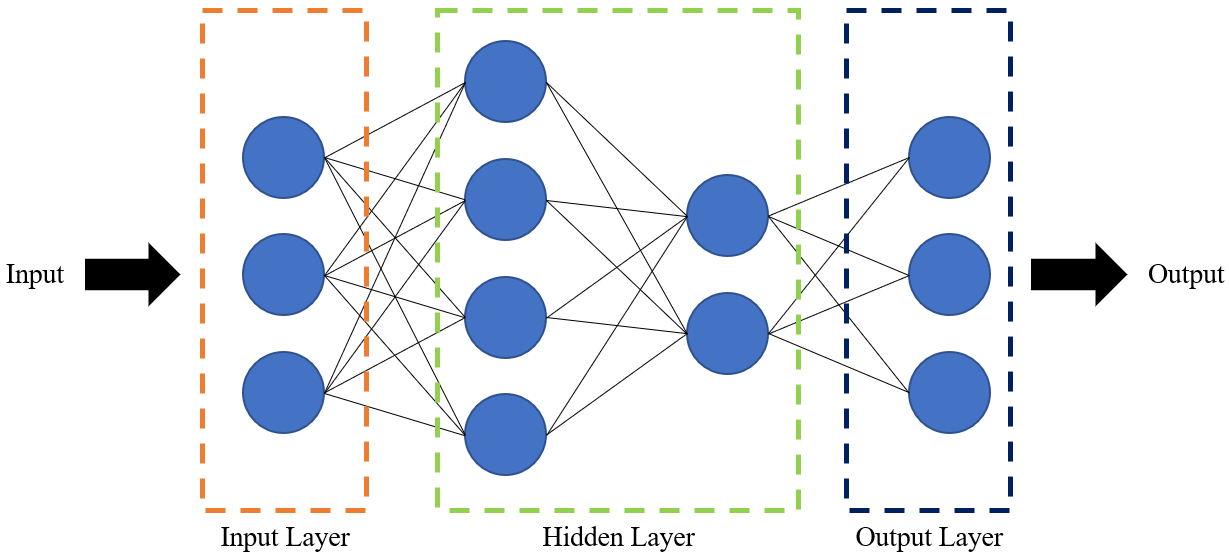
\includegraphics[width=0.6\textwidth]{Figures/Application To Deep Learning/DNNarch.png}
  \caption{Model of fully-connected (feed-forward) \acrshort{dnn}}
  \label{fig:DNNarch}
\end{figure}

\subsection{DNN Architectures}

Current \acrshort{dnn} architectures are grouped into three types of architecture, depending on the fundamental primitive operation being performed. These are Convolutional Neural Networks (\acrshort{cnn}), Recurrent Neural Networks (\acrshort{rnn}) and Unsupervised Pretrained Networks (\acrshort{upt}). 

\subsubsection{Convolutional Neural Networks (CNN)}
Convolutional Neural Networks can extract features from data via the convolution operation, being mainly used for image and object recognition and sound analysis. This type of architecture excels when there is some structure in the input data, that is, the data contains sets of specific patterns, organized in a spatial manner, that the neural network can learn to recognize.

The \acrshort{cnn} architecture generally follows the following pattern: input layer, feature-extraction layers and classification layer. The input layer receives a form of three-dimensional data, usually an image with a specific height and width and a depth value (representing color or intensity). The feature extraction layers perform higher-order features extract from the input, generally by performing patterns of convolution layers and pooling layers. Finally, the classification layer is a vector of size \textit{N}, where each output represents a score of prediction confidence for the input to be of a given output class.

Three common datasets used to compare and analyse the \acrshort{cnn}  performance are MNIST~\cite{lecun_yann_and_cortes_corinna_mnist_1999}, CIFAR~ 10~\cite{krizhevsky_learning_2009} and ImageNet~\cite{deng_imagenet_2009}, each with increased input complexity, number output classes and overall dataset size. MNIST consists of 70 000 images of handwritten digits 0 to 9, CIFAR10 consists of 60 000 images organized of 10 object and animal classes, and ImageNet is a collection of 14 million images of 20 thousand different classes. 

\subsubsection{Recurrent Neural Networks (RNN)}

Recurrent Neural Networks have the added capability of sending information over time-steps. This characteristic allows this type of architecture to have parallel and sequential data modeling, not only recognizing features from each input but also allowing for the extraction of features from the sequences of inputs, modeling the time dimension. 

acrshort{rnn}s are used to model time-series, language, audio, and text since this type of data is inherently ordered and context-sensitive. acrshort{rnn}s contain feedback loops between the layers, in order for each layer to have insights about what comed before. The model prediction follows the general format presented in Equation \ref{eq:rnn}, where $y$ represents the model prediction and $x$ the model inputs. The equation reflects the influence of previous inputs for each output.
\begin{equation}
    \label{eq:rnn}
    y[n] = x[n] + ... + x[n-i]
\end{equation}

The primitive that compose the feature extraction of \acrshort{rnn} models are LSTM - Long Short Term Memory. This type of layer unit has three gates - input, output and forget gates. The content of each LSTM is moduled by the input and forget gates; this change reflects on the value stored at the memory cell. If both gates are closed, the memory content remains unmodified between the current time-step and the following. The LSTM structure allows for information to be retained/forgotten on the memory cell across different time-steps.


\subsubsection{Unsupervised Pre-trained Networks (UPN)}
Unsupervised Pretrained Networks is a category of \acrshort{dnn} architectures that encompasses architectures such as autoencoders and generative adversarial networks (\acrshort{gan}s). This class of \acrshort{dnn} architecture departs from the previous ones, by learning in an unsupervised manner, meaning that the input data given to the network is not previously labeled. This introduces an extra degree of learning freedom by allowing the network to identify and recognize patterns that distinguish the output classes the most.

Autoencoders are used to learn efficient data codings and can be applied for dimensionality reduction or augmentation. Autoencoders allow for the reduction of noise in a signal or to perform a resolution increase on an image. \acrshort{gan}s can be used to perform sound and video synthesis from images or text using two neural networks in parallel - a discriminator and a generative network. First, the generative network creates a synthesized output from the given input given. Then the discriminator network tries to classify the input as real or synthesized, providing the classification to the generative network. With this data loop, the generative network updates their weights to fit best what is described as real data.


\subsection{Training and Inference}

The mathematical description of the \acrshort{dnn} training process, (see Equation \ref{eq:loss}), is equivalent to treating the network as a loss function $L$, where inputs $X$, outputs $Y$ and the network's parameters weights - $W$ and bias $b$ are function arguments. The training session's objective is to optimize the in-network parameters  $W$ (weights) and $b$ (bias) to minimize the overall loss.

\begin{equation}
    \label{eq:loss}
    (W,b) = \arg\min_{W} L(X,Y,W,b)
\end{equation}

The \acrshort{dnn} training is an iterative process, where at the end of each iteration, a loss value is computed, and the set of in-network parameters is updated. This loss value represents how well are the input parameters being modeled by the network. As the number of training iterations increases, the loss value reduces and converges to a minimum, at which the model accuracy prediction will be at its maximum. At this point, the training session can be stopped.

The most common method for the parameters update is the Stochastic Gradient Descent (\acrshort{sgd}) algorithm (see Equation \ref{eq:update}), an iterative algorithm that, after processing mini-batches of the training data, computes new weights and bias for each neuron. 

\begin{equation}
    \label{eq:update}
    W_{i+1} \xleftarrow{} W_i - \alpha \sum_{n=1}^{m}\frac{\partial L}{\partial W_i}
\end{equation}

In Equation \ref{eq:update}, $m$ represents the number of mini-batches to run, $W_i$ is the current parameter, $W_{i+1}$ the update parameter, $\alpha$ the learning rate and $\frac{\partial L}{\partial W_i}$ the partial derivative of the loss function $L$ in order to the parameters. This last equation is obtained by applying the derivative chain rule in a backward-cascade fashion with respect to inputs, outputs, and parameters of each \acrshort{dnn} layer.

Each iteration of the training process is composed of a forward and backward data propagation. On the forward propagation, the loss function for the current in-network parameters is evaluated, computing the loss value. By performing the backward propagation, the partial derivative $\frac{\partial L}{\partial W_i}$ of each of the parameters is obtained to apply the \acrshort{dnn} algorithm . 

The inference (or prediction) process corresponds to performing a forward propagation, with the intended input, on a previously trained neural network. At the output layer, a set of values (or probabilities) is computed, corresponding to the model's prediction to the given inputs.

\subsection{High-Level Libraries and Software Frameworks}

The popularization of \acrshort{gpu}s as the defacto \acrshort{dnn}s execution device comes at the cost of the availability of high-level libraries and frameworks from device manufacturers and other software houses. The available \acrshort{gpu} libraries implement the underlying mathematical operations performed during the \acrshort{dnn}s, while the frameworks operate on the execution of \acrshort{dnn}s by masking the complexity of creating, training and using these models~\cite{jain_performance_2019}.

The most used libraries are cuBLAS and cuDNN, by NVIDIA and rocBLAS and MIOpen, by AMD that implement the most optimize versions of matrix multiplication, convolution, and other kinds of mathematical operations to be used on the \acrshort{dnn} models. For the frameworks, TensorFlow and PyTorch are open-source frameworks developed by Google and Facebook, respectively that allow for easy implementation of the models in \acrshort{gpu}s.

%%%%%%%%%%%%%%%%%%%%%%%%%%%%%%%%%%%%%%%%%%%%%%%%%%%%%%%%%%%%%%%%%%%%%%%%
\section{DNN Performance and Energy Efficiency Improvement}
\label{section:DNN_conventional}

\acrshort{dnn} are usually characterized by significant computational burdens, particularly when considering the training of very deep and complex networks that deal with high dimensional data, such as images and videos. For such purpose, researchers (and data scientists, in general) often rely on accelerators, such as \acrshort{gpu}, to cope with the associated computational burden and reduce the training time. As a result, \acrshort{gpu} are now commonly deployed on most supercomputers, data centers and other computational infrastructures related to the development of artificial intelligence algorithms.

Additionally, several software frameworks, algorithms and techniques have been proposed to manage and optimize the execution of  \acrshort{dnn} on \acrshort{gpu} (e.g., Mittal~\cite{mittal_survey_2019}). However, most optimization techniques neglect the training phase's energy impact, usually resulting in considerable costs. 

To overcome this problem, researchers have also explored other solutions that allow mitigating the energy impact of neural network training. One particular and common approach relies on the use of low-precision arithmetic (e.g., Nabavinejad~\cite{nabavinejad_coordinated_2019}), eventually trading network accuracy with increased processing performance and lower energy consumption.

Researchers have also looked at alternative approaches, such as exploiting \acrshort{dvfs} on both the inference and training phases. In fact, by carefully selecting the used voltage-frequency (V-F) levels, significant energy savings can be obtained, although depending on the considered \acrshort{dnn} architecture and computing  device~\cite{tang_impact_2019}. This is achieved by a careful balance between the performance and power consumption of the different \acrshort{gpu} components  (particularly the core and global memory) to minimize stalls in the compute cores. In fact, not only can \acrshort{dvfs} be used to decrease the power consumption, but it can also boost the system performance~\cite{tang_impact_2019}, by increasing the voltage and frequency levels (as long as the GPU total power envelope and thermal limits are not surpassed).

%Nevertheless, as discussed, most state-of-the-art works only consider tightly coupled V-F levels, which are often predefined by GPU manufacturers and neglect the voltage margin that is usually introduced to guarantee fail-safe designs well as its variation with the kernel instruction sequence and the corresponding use of specific \acrshort{gpu} components. 


Supported on the performed \acrshort{gpu} characterization to non-conventional V-F pairs, this work continues by exploring the impact of these configurations on the \acrshort{cnn}s layers and training and inference.

%%%%%%%%%%%%%%%%%%%%%%%%%%%%%%%%%%%%%%%%%%%%%%%%%%%%%%%%%%%%%%%%%%%%%%%%
\section{Non-conventional V-F on CNNs}
\label{section:baseline}

\subsection{CNN Layer Characterization}

\subsubsection{Convolution Layers}

\subsubsection{Fully-Connected Layers}

\subsection{Error Analysis}

\subsubsection{Convolution Layers}

\subsubsection{Fully-Connected Layers}


%%%%%%%%%%%%%%%%%%%%%%%%%%%%%%%%%%%%%%%%%%%%%%%%%%%%%%%%%%%%%%%%%%%%%%%%
\section{Complete CNNs training with non-conventional V-F}
\label{section:enhanced}

\subsection{Experimental Setup}



\subsection{Feasibility Assessment}
Vou mostrar que treinar com estas settings nao estraga accuracy

\subsection{Performance and energy optimization}

\section{Summary}
% % ----------------------------------------------------------------------
% \subsection{Figures}
% \label{subsection:figures}

% Insert your section material and possibly a few figures...

% Make sure all figures presented are referenced in the text!


% % ----------------------------------------------------------------------
% \subsubsection{Images}
% \label{subsection:images}

% \begin{figure}[!htb]
%   \centering
%   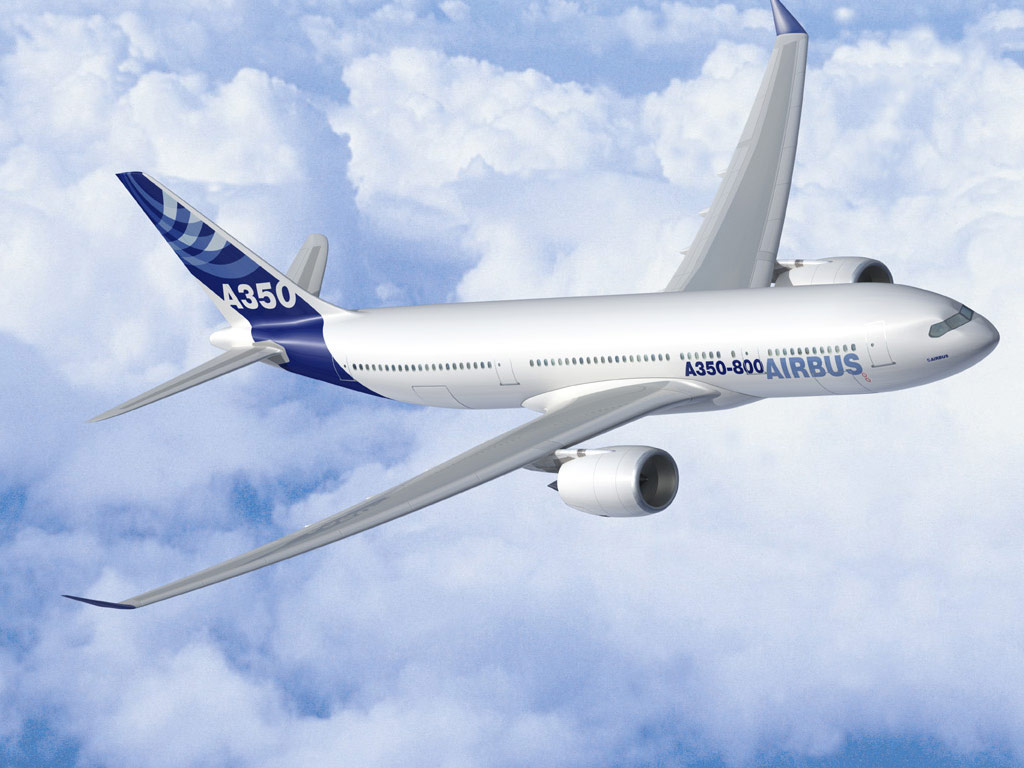
\includegraphics[width=0.25\textwidth]{Figures/Airbus_A350.jpg}
%   \caption[Caption for figure in TOC.]{Caption for figure.}
%   \label{fig:airbus1}
% \end{figure}

% \begin{figure}[!htb]
%   \begin{subfigmatrix}{2}
%     \subfigure[Airbus A320]{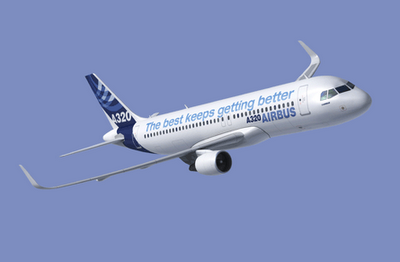
\includegraphics[width=0.49\linewidth]{Figures/Airbus_A320_sharklets.png}}
%     \subfigure[Bombardier CRJ200]{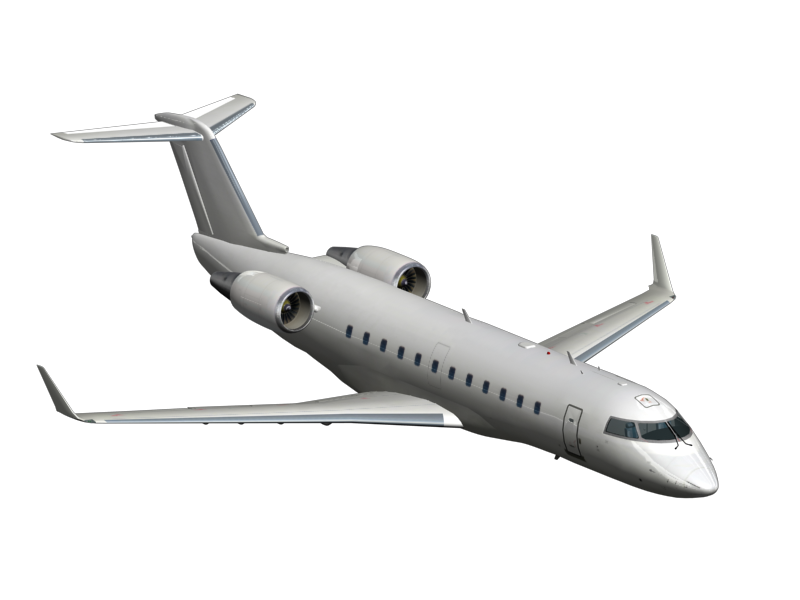
\includegraphics[width=0.49\linewidth]{Figures/Bombardier_CRJ200.png}}
%   \end{subfigmatrix}
%   \caption{Some aircrafts.}
%   \label{fig:aircrafts}
% \end{figure}

% Make reference to Figures \ref{fig:airbus1} and \ref{fig:aircrafts}.

% By default, the supported file types are {\it .png,.pdf,.jpg,.mps,.jpeg,.PNG,.PDF,.JPG,.JPEG}.

% See \url{http://mactex-wiki.tug.org/wiki/index.php/Graphics_inclusion} for adding support to other extensions.


% % ----------------------------------------------------------------------
% \subsubsection{Drawings}
% \label{subsection:drawings}

% Insert your subsection material and for instance a few drawings...

% The schematic illustrated in Fig.~\ref{fig:algorithm} can represent some sort of algorithm.

% \begin{figure}[!htb]
%   \centering
%   \scriptsize
% %  \footnotesize 
% %  \small
%   \setlength{\unitlength}{0.9cm}
%   \begin{picture}(8.5,6)
%     \linethickness{0.3mm}

%     \put(3,6){\vector(0,-1){1}}
%     \put(3.5,5.4){$\bf \alpha$}
%     \put(3,4.5){\oval(6,1){}}
%     %\put(0,4){\framebox(6,1){}}
%     \put(0.3,4.4){Grid Generation: \quad ${\bf x} = {\bf x}\left({\bf \alpha}\right)$}

%     \put(3,4){\vector(0,-1){1}}
%     \put(3.5,3.4){$\bf x$}
%     \put(3,2.5){\oval(6,1){}}
%     %\put(0,2){\framebox(6,1){}}
%     \put(0.3,2.4){Flow Solver: \quad ${\cal R}\left({\bf x},{\bf q}\left({\bf x}\right)\right) = 0$}

%     \put(6.0,2.5){\vector(1,0){1}}
%     \put(6.4,3){$Y_1$}

%     \put(3,2){\vector(0,-1){1}}
%     \put(3.5,1.4){$\bf q$}
%     \put(3,0.5){\oval(6,1){}}
%     %\put(0,0){\framebox(6,1){}}
%     \put(0.3,0.4){Structural Solver: \quad ${\cal M}\left({\bf x},{\bf q}\left({\bf x}\right)\right) = 0$}

%     \put(6.0,0.5){\vector(1,0){1}}
%     \put(6.4,1){$Y_2$}

%     %\put(7.8,2.5){\oval(1.6,5){}}
%     \put(7.0,0){\framebox(1.6,5){}}
%     \put(7.1,2.5){Optimizer}
%     \put(7.8,5){\line(0,1){1}}
%     \put(7.8,6){\line(-1,0){4.8}}
%   \end{picture}
%   \caption{Schematic of some algorithm.}
%   \label{fig:algorithm}
% \end{figure}


% % ----------------------------------------------------------------------
% \subsection{Equations}
% \label{subsection:equations}

% Equations can be inserted in different ways.

% The simplest way is in a separate line like this

% \begin{equation}
%   \frac{{\rm d} q_{ijk}}{{\rm d} t} + {\cal R}_{ijk}({\bf q}) = 0 \,.
% \label{eq:ode}
% \end{equation}

% If the equation is to be embedded in the text. One can do it like this ${\partial {\cal R}}/{\partial {\bf q}}=0$.

% It may also be split in different lines like this

% \begin{eqnarray}
%   {\rm Minimize}   && Y({\bf \alpha},{\bf q}({\bf \alpha}))            \nonumber           \\
%   {\rm w.r.t.}     && {\bf \alpha} \,,                                 \label{eq:minimize} \\
%   {\rm subject~to} && {\cal R}({\bf \alpha},{\bf q}({\bf \alpha})) = 0 \nonumber           \\
%                   &&       C ({\bf \alpha},{\bf q}({\bf \alpha})) = 0 \,. \nonumber
% \end{eqnarray}

% It is also possible to use subequations. Equations~\ref{eq:continuity}, \ref{eq:momentum} and \ref{eq:energy} form the Naver--Stokes equations~\ref{eq:NavierStokes}.

% \begin{subequations}
%     \begin{equation}
%     \frac{\partial \rho}{\partial t} + \frac{\partial}{\partial x_j}\left( \rho u_j \right) = 0 \,,
%     \label{eq:continuity}
%     \end{equation}
%     \begin{equation}
%     \frac{\partial}{\partial t}\left( \rho u_i \right) + \frac{\partial}{\partial x_j} \left( \rho u_i u_j + p \delta_{ij} - \tau_{ji} \right) = 0, \quad i=1,2,3 \,,
%     \label{eq:momentum}
%     \end{equation}
%     \begin{equation}
%         \frac{\partial}{\partial t}\left( \rho E \right) + \frac{\partial}{\partial x_j} \left( \rho E u_j + p u_j - u_i \tau_{ij} + q_j \right) = 0 \,.
%     \label{eq:energy}
%     \end{equation}
% \label{eq:NavierStokes}%
% \end{subequations}


% % ----------------------------------------------------------------------
% \subsection{Tables}
% \label{section:tables}

% Insert your subsection material and for instance a few tables...

% Make sure all tables presented are referenced in the text!

% Follow some guidelines when making tables:

% \begin{itemize}
%   \item Avoid vertical lines
%   \item Avoid “boxing up” cells, usually 3 horizontal lines are enough: above, below, and after heading
%   \item Avoid double horizontal lines
%   \item Add enough space between rows
% \end{itemize}

% \begin{table}[!htb]
%   \renewcommand{\arraystretch}{1.2} % more space between rows
%   \centering
%   \begin{tabular}{lccc}
%     \toprule
%     Model           & $C_L$ & $C_D$ & $C_{M y}$ \\
%     \midrule
%     Euler           & 0.083 & 0.021 & -0.110    \\
%     Navier--Stokes  & 0.078 & 0.023 & -0.101    \\
%     \bottomrule
%   \end{tabular}
%   \caption[Table caption shown in TOC.]{Table caption.}
%   \label{tab:aeroCoeff}
% \end{table}

% Make reference to Table \ref{tab:aeroCoeff}.

% Tables \ref{tab:memory} and \ref{tab:multipleColumns} are examples of tables with merging columns:

% \begin{table}[!htb]
%   \renewcommand{\arraystretch}{1.2} % more space between rows
%   \centering
%   \begin{tabular}[]{lrr}
%     \toprule
%                 & \multicolumn{2}{c}{\underline{Virtual memory [MB]}} \\
%                 & Euler       & Navier--Stokes \\
%     \midrule
%       Wing only &  1,000      &    2,000       \\
%       Aircraft  &  5,000      &   10,000       \\
%       (ratio)   & $5.0\times$ & $5.0\times$    \\
%     \bottomrule
%   \end{tabular}
%   \caption{Memory usage comparison (in MB).}
%   \label{tab:memory}
% \end{table}

% \begin{table}[!htb]
%   \centering
%   \renewcommand{\arraystretch}{1.2} % more space between rows
%   \begin{tabular}{@{}rrrrcrrr@{}} % remove space to the vertical edges @{}...@{}
%     \toprule
%       & \multicolumn{3}{c}{$w = 2$} & \phantom{abc} & \multicolumn{3}{c}{$w = 4$} \\
%     \cmidrule{2-4}
%     \cmidrule{6-8}
%       & $t=0$ & $t=1$ & $t=2$ && $t=0$ & $t=1$ & $t=2$ \\
%     \midrule
%       $dir=1$
%       \\
%       $c$ &  0.07 &  0.16 &  0.29 &&  0.36 &  0.71 &   3.18 \\
%       $c$ & -0.86 & 50.04 &  5.93 && -9.07 & 29.09 &  46.21 \\
%       $c$ & 14.27 &-50.96 &-14.27 && 12.22 &-63.54 &-381.09 \\
%       $dir=0$
%       \\
%       $c$ &  0.03 &  1.24 &  0.21 &&  0.35 & -0.27 &  2.14 \\
%       $c$ &-17.90 &-37.11 &  8.85 &&-30.73 & -9.59 & -3.00 \\
%       $c$ &105.55 & 23.11 &-94.73 &&100.24 & 41.27 &-25.73 \\
%     \bottomrule
%   \end{tabular}
%   \caption{Another table caption.}
%   \label{tab:multipleColumns}
% \end{table}

% An example with merging rows can be seen in Tab.\ref{tab:multipleRows}.

% \begin{table}[!htb]
%   \renewcommand{\arraystretch}{1.2} % more space between rows
%   \centering
%   \begin{tabular}{ccccc}
%     \toprule
%       \multirow{2}{*}{ABC} & \multicolumn{4}{c}{header} \\
%       \cmidrule{2-5} & 1.1 & 2.2 & 3.3 & 4.4 \\
%     \midrule
%       \multirow{2}{*}{IJK} & \multicolumn{2}{c}{\multirow{2}{*}{group}} & 0.5 & 0.6 \\
%       \cmidrule{4-5}       & \multicolumn{2}{c}{}                       & 0.7 & 1.2 \\
%     \bottomrule
%   \end{tabular}
%   \caption{Yet another table caption.}
%   \label{tab:multipleRows}
% \end{table}

% If the table has too many columns, it can be scaled to fit the text widht, as in Tab.\ref{tab:scale}.
% \begin{table}[!htb]
%   \renewcommand{\arraystretch}{1.2} % more space between rows
%   \centering
%   \resizebox*{\textwidth}{!}{%
%     \begin{tabular}[]{lcccccccccc}
%       \toprule
%         Variable &  a  &  b  &  c  &  d  &  e  &  f  &  g  &  h  &  i  &  j  \\
%       \midrule
%         Test 1   &  10,000 &  20,000 &  30,000 &  40,000 &  50,000 &  60,000 &  70,000 &  80,000 &  90,000 & 100,000 \\
%         Test 2   &  20,000 &  40,000 &  60,000 &  80,000 & 100,000 & 120,000 & 140,000 & 160,000 & 180,000 & 200,000 \\
%       \bottomrule
%     \end{tabular}
%   }%
%   \caption{Very wide table.}
%   \label{tab:scale}%
% \end{table}


% % ----------------------------------------------------------------------
% \subsection{Mixing}
% \label{section:mixing}

% If necessary, a figure and a table can be put side-by-side as in Fig.\ref{fig:side_by_side}

% \begin{figure}[!htb]
%   \begin{minipage}[b]{0.60\linewidth}
%     \centering
%     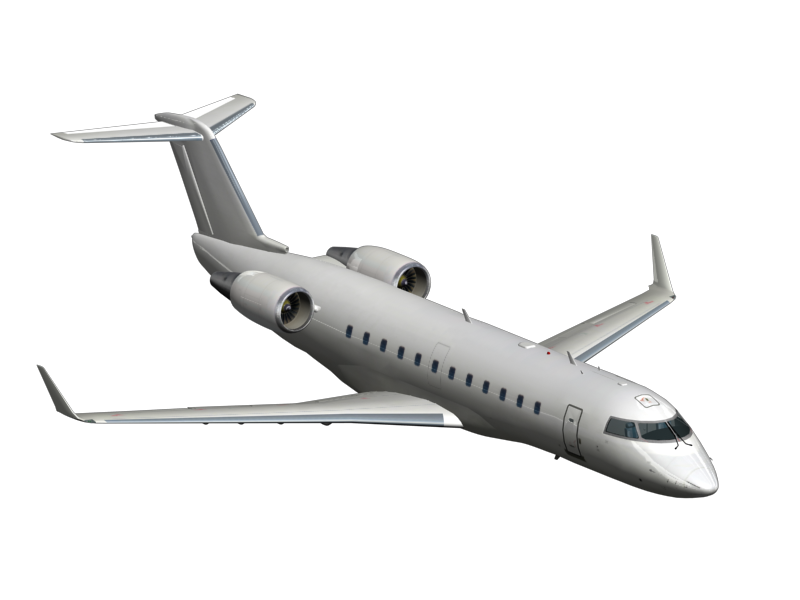
\includegraphics[width=\linewidth]{Figures/Bombardier_CRJ200}
%   \end{minipage}%
%   \begin{minipage}[b]{0.30\linewidth}
%     \centering
%     \begin{tabular}[b]{lll}
%       \toprule
%         \multicolumn{3}{c}{Legend} \\
%       \midrule
%         A & B & C \\
%         0 & 0 & 0 \\
%         0 & 1 & 0 \\
%         1 & 0 & 0 \\
%         1 & 1 & 1 \\
%       \bottomrule
%     \end{tabular}
%     \vspace{5em}
%   \end{minipage}
% \caption{Figure and table side-by-side.}
% \label{fig:side_by_side}
% \end{figure}

